For one dimensional data, the evaluation covers the following tasks:

\begin{itemize}
	\item Find a structure for recursive model index empirically.
	\item Compares the performance between baseline model, recursive model and traditional B-Tree.
\end{itemize}

\subsection{Dataset}

For one dimensional case, we manually generate two columns of the data:

\begin{itemize}
	\item The first column contains the keys $X$, which is randomly sampled from a given distribution.
	\item Then we assign the keys into different pages according to a preset parameter $N_{page}$ for page size. Specifically, the first $N_{page}$ keys will be assigned into the first page, the second $N_{page}$ keys will be assigned into the second page and so on so forth. After the assignments, we set the second column $Y$ to be the page index of the corresponding $x$.
\end{itemize}

\textbf{Small Lognormal Distributed Data} We first generate $10,000$ data points where $X$ is from a lognormal distribution $\text{Lognormal}(0, 4)$. 

\begin{table}
	\centering
	\begin{tabular}{||c | c | c | c | c | c||}
		\hline
		Name& root model & 2nd model & No. of 2nd models & 3rd model & No. of 3rd models \\ [0.5ex] 
		\hline
		\hline
		Setting 1  & FCN& FCN& 200 & FCN& 2000\\
		\hline
		Setting 2  & FCN& FCN& 200 & FCN& 4000\\
		\hline
		Setting 3  & FCN& FCN& 200 & FCN& 6000\\
		\hline
		Setting 4  & FCN& FCN& 400 & FCN& 2000\\ 
		\hline
		Setting 5  & FCN& FCN& 400 & FCN& 4000\\
		\hline
		Setting 6  & FCN& FCN& 400 & FCN& 6000\\
		\hline 
		Setting 7  & FCN& FCN& 600 & FCN& 2000\\
		\hline 
		Setting 8  & FCN& FCN& 600 & FCN& 4000\\
		\hline 
		Setting 9  & FCN& FCN& 600 & FCN& 6000\\
		\hline
		Setting 10 & LR & LR& 200 & LR& 2000\\
		\hline
		Setting 11 & LR & LR& 200 & LR& 4000\\
		\hline
		Setting 12 & LR & LR& 200 & LR& 6000\\
		\hline
		Setting 13 & LR & LR& 400 & LR& 2000\\ 
		\hline
		Setting 14 & LR & LR& 400 & LR& 4000\\ 
		\hline
		Setting 15 & LR & LR& 600 & LR& 2000\\ 
		\hline
		Setting 16 & LR & LR& 600 & LR& 4000\\ 
		\hline
		Setting 17 & LR & LR& 600 & LR& 6000\\ 
		\hline
		Setting 18 & LR & LR& 400 & LR& 6000\\ 
		\hline
		Setting 19 & LR & FCN& 200 & FCN& 4000\\
		\hline
		Setting 20 & FCN& FCN& 200 & LR& 4000\\
		\hline 
		Setting 21 & FCN& LR& 200 & LR& 4000\\
		\hline 
		Setting 22 & LR & FCN& 200 & LR& 4000\\
		\hline 
		Setting 23 & FCN& LR& 200 & LR& 4000\\
		\hline
		Setting 24 & FCN& LR& 200 & LR& 4000\\
		\hline
		\hline
	\end{tabular}
	\label{small_lognormal_settings}
	\caption{Structures of recursive models for small lognormal data}
\end{table}

\begin{center}
	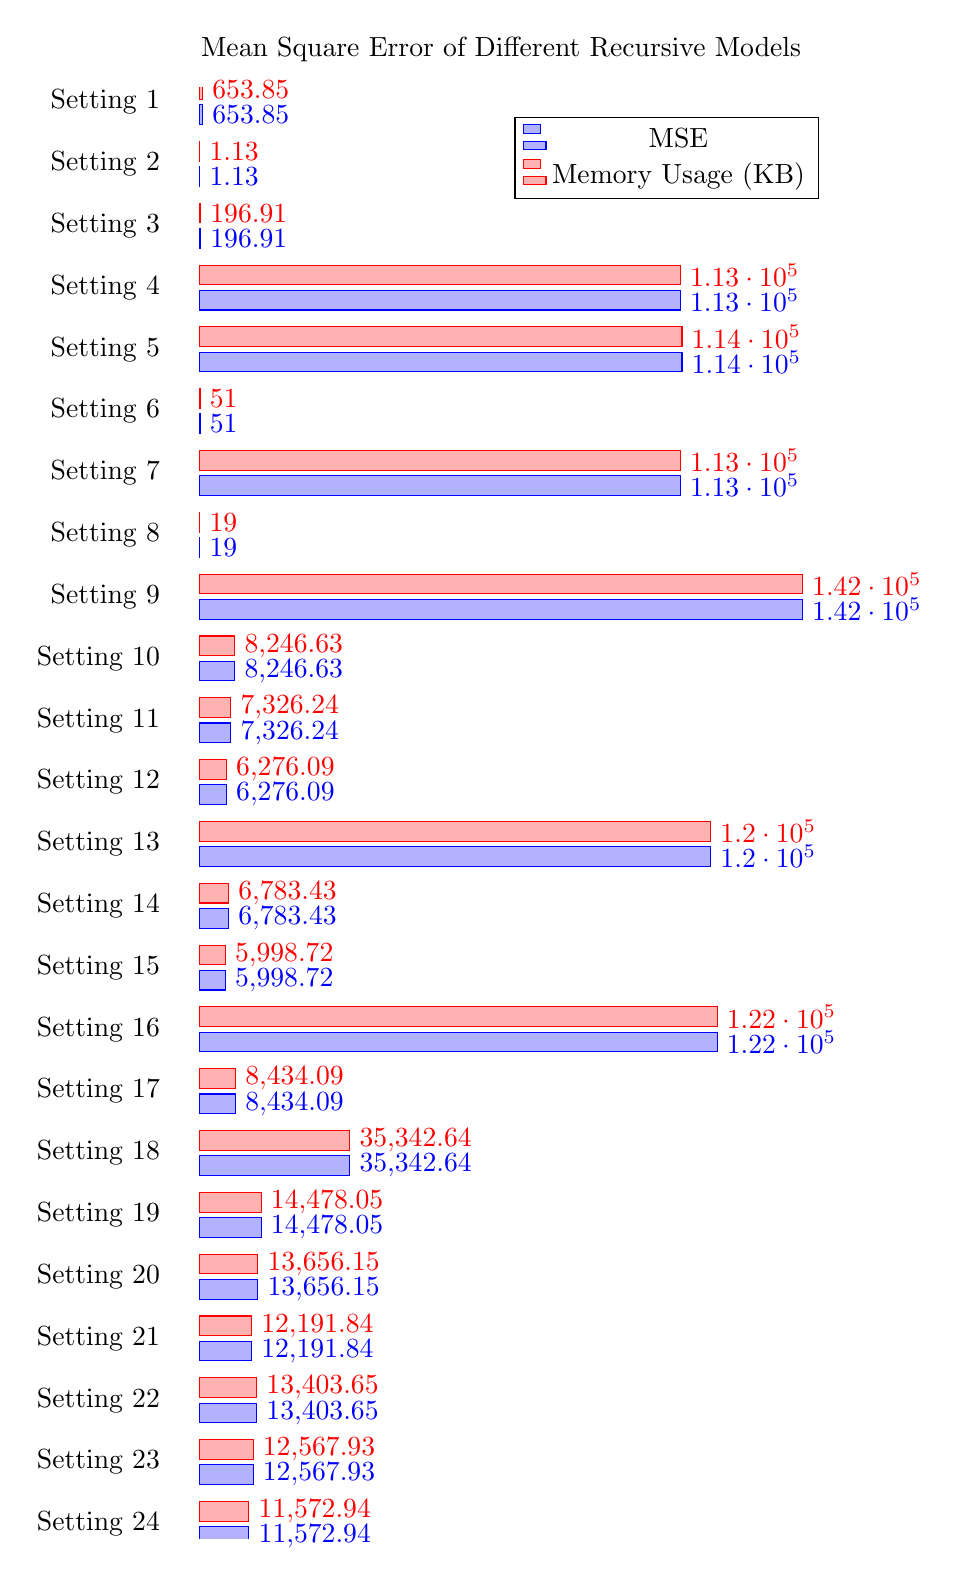
\begin{tikzpicture}
		\begin{axis}[title  = Mean Square Error of Different Recursive Models,
				xbar,
				y axis line style = { opacity = 0 },
				axis x line= none,
				ytick             = data,
				tickwidth = 0pt,
				enlarge y limits  = 0.01,
				enlarge x limits  = 0.05,
				bar width=2.5mm,
				height=20cm,
				width=10cm,
				symbolic y coords = {Setting 24, Setting 23, Setting 22, Setting 21, Setting 20, Setting 19, Setting 18, Setting 17, Setting 16, Setting 15, Setting 14, Setting 13, Setting 12, Setting 11, Setting 10, Setting 9, Setting 8, Setting 7, Setting 6, Setting 5, Setting 4, Setting 3, Setting 2, Setting 1},
				nodes near coords,
			]
			\addplot coordinates { 
			    (653.8536667,Setting 1)
				(1.134166667,Setting 2)
				(196.9116667,Setting 3)
				(113246.196,Setting 4) 
				(113652.3212,Setting 5)
				(51.00183333,Setting 6)
				(113246.2647,Setting 7)
				(18.99766667,Setting 8)
				(142041.6877,Setting 9)
				(8246.633985,Setting 10) 
				(7326.238372,Setting 11)
				(6276.09111,Setting 12)
				(120427.9247,Setting 13)
				(6783.428749,Setting 14)
				(5998.720313,Setting 15) 
				(121932.5051,Setting  16)
				(8434.091306,Setting 17)
				(35342.6365,Setting 18)
				(14478.05283,Setting 19)
				(13656.1507,Setting 20) 
				(12191.8397,Setting 21)
				(13403.64758,Setting 22)
				(12567.93278,Setting 23)
				(11572.93555,Setting 24)};
			\addplot coordinates {
				(653.8536667,Setting 1)
				(1.134166667,Setting 2)
				(196.9116667,Setting 3)
				(113246.196,Setting 4) 
				(113652.3212,Setting 5)
				(51.00183333,Setting 6)
				(113246.2647,Setting 7)
				(18.99766667,Setting 8)
				(142041.6877,Setting 9)
				(8246.633985,Setting 10) 
				(7326.238372,Setting 11)
				(6276.09111,Setting 12)
				(120427.9247,Setting 13)
				(6783.428749,Setting 14)
				(5998.720313,Setting 15) 
				(121932.5051,Setting  16)
				(8434.091306,Setting 17)
				(35342.6365,Setting 18)
				(14478.05283,Setting 19)
				(13656.1507,Setting 20) 
				(12191.8397,Setting 21)
				(13403.64758,Setting 22)
				(12567.93278,Setting 23)
				(11572.93555,Setting 24)};
			\legend{MSE, Memory Usage (KB)}
		\end{axis}
	\end{tikzpicture}
\end{center}

\textbf{Various Distributions and Sizes} After the search process for a recursive model, we then conduct experiments on several different distributions and sizes datasets. During this process, we use the following settings:

\textbf{Large Lognormal Distributed Data} The last dataset that we used is a large dataset that contains 190 million key value pairs that are distributed under lognormal distribution.